\documentclass{beamer}
\usetheme{metropolis} % Use metropolis theme

\usepackage[utf8]{inputenc}
\usepackage[T1]{fontenc}
\usepackage[british]{babel}
\usepackage[autostyle, english = british]{csquotes}
\usepackage[%
  backend=biber,
  doi=false,
  url=false,
  isbn=false,
  eprint=false,
  style=authoryear,
  hyperref=true,
  maxnames=2,
  minnames=1,
  maxbibnames=99,
  firstinits,
  uniquename=init]{biblatex}
\addbibresource{../bibliography.bib}

\usepackage{caption}
\usepackage{xpatch}
\usepackage{bm}
\usepackage{amsmath}
\usepackage{mathtools} % for \mathclap
\usepackage{varioref}
\usepackage{siunitx}
\usepackage{hyperref}
\usepackage[noabbrev]{cleveref}
\newcommand{\creflastconjunction}{, and\nobreakspace} % use Oxford comma
\usepackage{todonotes}
\usepackage{phaistos}
\usepackage{multimedia}
\usepackage{tikz}
\usetikzlibrary{arrows, positioning, shapes.geometric}
\usetikzlibrary{calc}
\graphicspath{{../../figures/}}

\newcommand{\cn}{\textbf{TODO: Citation}}

\title{Data-Driven Models for Zebrafish Motion\\IDP kick-off}
\author{Lukas Krenz}
\date{January 12, 2018} 
\institute{TUM}

\begin{document}
\maketitle
\begin{frame}{What \textit{\&} Why?}
Collaboration with Couzin Lab (Max Plank Institute for Ornithology/University of Konstanz)

Advisers: Dr.\ Jacob Davidson (Konstanz), Nicola Rieke (CAMP)

Supervisor: Prof.\ Dr.\ Nassir Navab

Goals:
\begin{enumerate}
\item Compare three models for motion of juvenile zebrafish (only roughly 1cm long)
\item Not a tracking project, rather data-driven modelling/machine learning
\item Example use case: virtual reality for fish
\end{enumerate}
\end{frame}
\begin{frame}{Zebrafish: Burst-and-coast Motion} 
    \begin{figure}[H]
    \centering
    \movie[width=0.66\textwidth, height=0.66\textwidth, autostart,, loop, poster]{}{motion_experiment.mp4}
    \caption{Example of zebrafish motion}
    \label{fig:calovi-sim}
  \end{figure}
\end{frame}

\begin{frame}
  \frametitle{Modeling Fish Motion}
Data: Roughly 100k kicks from 10 experiments with 2 fish swimming, each 1h long

Videos already tracked!

Segmentation into kicks as preprocessing step

Model Input: Distance and angle between fish and wall, distance and angles between both fish

Later: Data from more timesteps

Model Output: Heading change of one fish

One model per fish
\end{frame}

\begin{frame}{First Model: Force Based (Calovi et al)}
Following ideas from \textit{Disentangling and modeling interactions in fish with burst-and-coast swimming}, arXiv, 2017, {\tiny{Calovi, D.S., Litchinko, A., Lecheval, V., Lopez, U., Escudero, A.P., Chaté, H., Sire, C. and Theraulaz, G.}} 

\begin{enumerate}
\item Discrete model, model heading change $\delta \phi$ for kicks
\item Decision process only uses current status
\item Force based, stochastic model
\item Symmetry constraints 
\end{enumerate}

Full model:
\begin{align*}
  \label{eq:calovi-model}
  \delta \phi &= \delta \phi_r (r_w) + \delta \phi_w (r_w, \theta_w) + \delta \phi_\text{Att} (d, \psi, \Delta \phi) + \delta \phi_\text{Ali}  (d, \psi, \Delta \phi) \\
  &= \text{noise} + \text{wall avoidance} + \text{attraction} + \text{alignment}
\end{align*}
with: $r_w$ distance to wall, $\theta_w$ angle towards wall,\\ $d$ distance between both fish, $\psi$ viewing angle and $\Delta \phi$ relative angle
\end{frame}

\begin{frame}
  \frametitle{Calovi - Wall Fit}
{\centering
\includegraphics[clip, width=1.09\linewidth]{wall_fit.pdf}
}
\only<1>{
\begin{align*}
  \delta \phi_w (r_w, \theta_w) &= f(r_w)O_w(\theta_w) \\
  f(r_w) &= \exp\left( -{(r_w/l_w)}^2 \right) \\
  O(\theta_w) &= \left(a_1 \sin(\theta_w) + a_2 \sin(2  \theta_w)  \right)  \left(1 +  b_1  \cos(\theta_w) + b_2 \cos(2  \theta_w) \right)
\end{align*}
$r_w$ distance to wall, $\theta_w$ angle towards wall
}
\only<2>{
%   Stable fixed points at -\ang{-90} and \ang{90} -> swimming parallel to wall
%   Unstable fixed points at \ang{-180}, and \ang{180} -> swimming away from wall
% TODO: Figure for fixed points
% %what about the one at 0°?
 \begin{columns}
   \begin{column}{0.5\textwidth}
  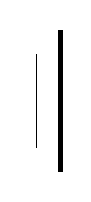
\begin{tikzpicture}[scale=0.3]
   \draw (3,-2)--(3,2); %fish
   \draw[ultra thick] (4,-3)--(4,3);
   \node[rotate=-90] at (3,-1) {\PHtunny};
 \end{tikzpicture}\qquad\qquad
  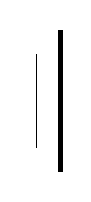
\begin{tikzpicture}[scale=0.3]
   \draw (3,-2)--(3,2); %fish
   \draw[ultra thick] (4,-3)--(4,3);
   \node[rotate=90] at (3,1) {\PHtunny};
 \end{tikzpicture}
 
\textbf{Stable fixed points}\\\ang{-90} and \ang{90}
   \end{column}
   \begin{column}{0.5\textwidth}
  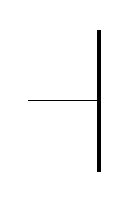
\begin{tikzpicture}[scale=0.3]
   \draw (0,0)--(3,0); % fish
   \draw[ultra thick] (3,-3)--(3,3);
   \node[rotate=180] at (1,0) {\PHtunny};
 \end{tikzpicture}\qquad\qquad
   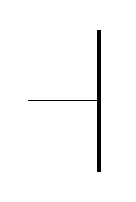
\begin{tikzpicture}[scale=0.3]
   \draw (0,0)--(3,0); % fish
   \draw[ultra thick] (3,-3)--(3,3);
   \node[rotate=0] at (3,0) {\PHtunny};
 \end{tikzpicture}

\textbf{Unstable fixed points}\\\ang{0}, \ang{-180} and \ang{180}  
   \end{column}
   
 \end{columns}
} 

\end{frame}

\begin{frame}
  \frametitle{Calovi - First simulation}
\begin{figure}[H]
    \centering
    \movie[width=0.66\textwidth, height=0.66\textwidth, autostart,, loop, poster]{}{wall_animation.mp4}
    \caption{First results for wall model}
    \label{fig:calovi-sim}
\end{figure}
\end{frame}

\begin{frame}
  \frametitle{Second model: Spatio-Temporal-Receptive Field}
 \begin{columns}
   \begin{column}{0.5\textwidth}
  \begin{tikzpicture}[scale=0.5]
   \draw[red] (3, 3)--(5,5);
   \draw[ultra thick] (0,0)--(0,5);
   %\draw (4,-3)--(4,3);
   \node[rotate=45] at (4.5,4.5) {\textcolor{red}\PHtunny};
   \node[rotate=90] at (2.5,2.5) {\PHtunny};
 \end{tikzpicture}

 \textbf{No memory}: Only current position, etc.
\end{column}~\begin{column}{0.5\textwidth}
  \begin{tikzpicture}[scale=0.5]
   \draw[red] (3, 3)--(5,5); % our fish
   \draw[ultra thick] (0,0)--(0,5); % wall
   \draw[gray] (2.5, 0)--(2.5,2.5);
   \node[rotate=45] at (4.5,4.5) {\textcolor{red}\PHtunny};
   \node[rotate=90] at (2.5,2.5) {\PHtunny};
   \node[rotate=90] at (2.5,0.5) {\textcolor{gray}\PHtunny};
 \end{tikzpicture}

 \textbf{Memory}: Current position and trace
   \end{column}
 \end{columns}
  Inspired by computational neuroscience

  Drop assumption that kick is influenced only by current surroundings
  
  Approximate forces by weighted sum over past environment influences (e.g.\ distances, angles)

  Linear model with memory
\end{frame}

\begin{frame}
  \frametitle{Third Model: Neural Network}
  Idea: Approximate environment forces with a neural network

  Time series data, strong autocorrelation

  Some evidence for non-linear effects in collective animal motion
  (e.g. in\ \textit{Inferring the structure and dynamics of interactions in schooling fish}, PNAS, 2011, {\tiny Katz, Y., Tunstrøm, K., Ioannou, C. C., Huepe, C., and Couzin, I. D.})

  Use models such as recurrent neural networks (e.g.\ LSTM, GRU) or causal convolutional networks
  
  Highly non-linear model with memory
\end{frame}

\begin{frame}
  \frametitle{Summary and timeline}
  \begin{itemize}
  \item Calovi: Linear model without memory
  \item Spatio-Temporal Receptive Field: Linear model with memory
  \item Neural Network: Non-linear model with memory 
  \end{itemize}

  \begin{block}{Timeline}
    Steps will be finished in roughly$\dots$
  \begin{description}
\item[2 weeks] Pre-processing and Calovi
\item[2 months] Linear Receptive Field
\item[3 months] Non-Linear Receptive Field (Neural Network)
  \end{description}
   
  \end{block}
  
\end{frame}

\section{Appendix}

\begin{frame}{Calovi - Only wall}
Consider no social component:
 \begin{equation*}
  \label{eq:calovi-wall_model}
  \delta \phi = \delta \phi_r (r_w) + \delta \phi_w (r_w, \theta_w)
\end{equation*}
Symmetry for wall influence:
\begin{equation*}
  \label{eq:calovi-wall-symmetry}
   \delta \phi_w (r_w, -\theta_w) =  - \delta \phi_w (r_w, \theta_w)
\end{equation*}
Split into force term $f(r_w)$ and odd function $O_r(\theta_w)$ 
\begin{equation*}
  \label{eq:calovi-wall-split}
  \delta \phi_w (r_w, \theta_w) = f(r_w)O_w(\theta_w)
\end{equation*}
\begin{align*}
  \label{eq:calovi-wall-force}
  f(r_w) &= \exp\left( -{(r_w/l_w)}^2 \right) \\
  O(\theta_w) &= \left(a_1 \sin(\theta_w) + a_2 \sin(2  \theta_w)  \right)  \left(1 +  b_1  \cos(\theta_w) + b_2 \cos(2  \theta_w) \right)
\end{align*}
\end{frame}

\end{document}